
\chapter[Introdução]{Introdução}
%\addcontentsline{toc}{chapter}{Introdução}
% ----------------------------------------------------------

\section{Motivação}

O problema de buscar o melhor caminho entre dois pontos tem uma grande importância em áreas como da engenharia e ciência, tais como rotear o tráfico de telefone, navegar por um labirinto ou mesmo definir o layout de trilhas impressas em uma placa eletrônica.

Busca de caminhos também tem uma grande importância no âmbito dos jogos digitais, onde um jogador compete ou coopera com uma inteligência artificial e é preciso chegar ao seu destino de forma competente, como por exemplo, jogos de tiro em primeira pessoa ou de estratégia em tempo real.

O valor de entretenimento do jogo pode ser drasticamente reduzido, quando os personagens não podem atravessar um mapa complexo de forma competente, podendo afetar a experiência de jogo ao deixar visível para o jogador a sua incapacidade de lidar com a busca de caminho de forma satisfatória.

Ainda é comum, em jogos digitais, termos mais de um agente de busca de caminho ao mesmo tempo no mesmo cenário, podendo ser muitas vezes muito custoso computacionalmente falando. Para isso vários desenvolvedores de jogos têm juntado esforços para desenvolver soluções de busca de caminho em ambientes de recursos escassos.\cite{Pontevia}

%\section{Justificativa}

Muitas abordagens para melhorar o desempenho ou diminuir o custo de métodos de busca de caminho tem sido desenvolvidos \cite{Ulysses}  \cite{Pollack} \cite{Timothy} \cite{WilliamMiller}. 

Ainda temos problemas de alto custo computacional, que para serem minimizados em alguns casos, acabamos sacrificando a certeza de melhor caminho por um melhor desempenho\cite{Botea}\cite{KORF199341}. Por isso iremos faremos uma análise e propor um modelo para otimizar alguma limitação do modelo, visando em principal o âmbito dos jogos digitais.

Qualquer problema que possa ser formulado em busca em grafos pode ser solucionado a partir de busca heurísticas. O exemplo mais comum que pode ser representado por um grafo é o PCV, outro exemplo típico é quebra-cabeça de deslizar, que consiste em um quadro que contem quadrados numerados e uma posição vazia (Conforme a Figura \ref{fig:GrafoBusca}). As operações permitidas são deslizar qualquer peça horizontalmente ou verticalmente adjacente a peça vazia para a posição vazia e o objetivo é rearranjar as peças a partir de uma configuração randômica com menor quantidade de movimentos. Encontrar a solução ótima para esse problema ou para o PCF é NP-Completo. \cite{Kar72} \cite{RatnerW86}

\begin{minipage}{\linewidth}
    \makebox[\linewidth][c]{
        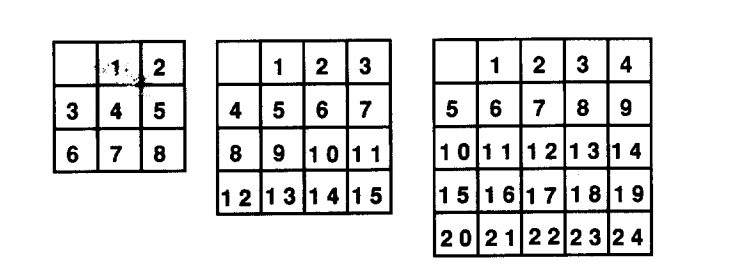
\includegraphics[keepaspectratio=true,scale=0.8]{ibagens/slide-puzzle.png}}
    \captionof{figure}{Quebra cabeça de deslizar \cite{KORF199341}}
    \label{fig:slide-puzzle}
\end{minipage}

Este cenário é a principal motivação deste trabalho que consiste implementar e mensurar resultados de uma solução para busca de melhor caminho entre dois pontos.

\section{Objetivos}

Este trabalho tem como objetivo verificar a aplicabilidade de paralelismo de AG para melhoria de precisão em busca heurística de caminhos. O ponto central é a definição de uma estrutura capaz de explorar as vantagens demonstradas no uso de AG com computação paralela e aplicá-las em um modelo de busca heurística de caminho que use AG para redução de custo de memória e processamento, já que para isto, estes tendem a sacrificar a certeza de encontrar a menor rota. 

\subsection{Objetivos Específicos}

Implementar o modelo de busca heurística com AG e mensurar os resultados. 

Aplicar um modelo de paralelização de AG. 

Combinar o modelo paralelo com o de busca e mensurar os resultados.

\section{Método de trabalho}

Primeiramente será desenvolvido uma bateria de testes de caminhos, com intuito de terem diferentes tamanhos, levando em consideração mapas com padrões de repetição e sem padrões de repetição, os mesmos serão modelados de forma bidimensional em arquivos de texto com caracteres para definir o ponto inicial (S), final (E), obstáculos (\#) e caminho livre (.).

Será implementada a busca heurística A* utilizando a linguagem C\# e .NET Framework da Microsoft, levando em consideração os arquivos de teste desenvolvidos como entrada, retornando se existe um caminho entre o ponto inicial e final, quanto tempo levou para encontrar o caminho e consumo de memoria para chegar na solução. 

Também será implementado um AG para utilizar em conjunto ao A*, também utilizando a linguagem C\# .NET, implementando o mesmo método proposto por Ulysses O. Santos \cite{Ulysses}. A implementação receberá  arquivos de testes de entrada contendo os mapas, os mesmos serão utilizado para testar a implementação do A* anteriormente, também retornando o tempo e consumo de memoria para chegar na solução. Os parâmetros para serem utilizados no AG serão:

Uma população inicial de 4 indivíduos

Critério de geração de descendentes em 50\%

Critério de mutação em 25\% 

Aptidão para 12 indivíduos

Por último, será implementado uma modificação do AG paralelo, como proposto por \cite{Alaoui}. Serão utilizadas N \textit{threads} para a separação das populações, ou seja, trabalhando com várias populações ao mesmo tempo, onde cada \textit{thread} fica responsável por uma, para depois mesclar os melhores indivíduos entre elas, esse sistema ira receber os mesmo arquivos de testes utilizados nas implementações anteriores, retornando informações de tempo e consumo de memória.

Será calcula a média de tempo e consumo de memória entre cada um dos testes. Todos os dados coletados serão comparados em forma de tabelas e gráficos, para demostrar os ganhos e perdas relativos de cada abordagem.

\section{Organização do trabalho}
Este trabalho é dividido em 4 capítulos. O primeiro capitulo faz uma introdução geral do problema, descrever os objetivos e a motivação para a resolução do problema proposto.

O segundo capitulo trata do problema de forma separada, mostrando o que existe na literatura para uma possível solução. Também explica de forma mais detalhada o funcionamento de dois exemplos de busca heurística, demostrando uma aplicação em um trabalho da literatura e dos algoritmos genéticos, explicando seu funcionamento e aplicação na literatura.
O terceiro capitulo é a proposta apresentada para a criação deste trabalho.
O quarto capitulo mostra o cronograma para a segunda parte do trabalho.
